\documentclass{beamer}

\mode<presentation>
{
  \usetheme{default}
  \setbeamertemplate{navigation symbols}{}
  \setbeamertemplate{footline}[frame number]
  \setbeamertemplate{items}[circle]
  \usecolortheme{seahorse}
}

\usepackage[english]{babel}
\usepackage[utf8]{inputenc}
\usepackage{times}
\usepackage[T1]{fontenc}
\usepackage{url}

\newcommand\topstrut{\rule{0pt}{2.6ex}}
\newcommand\bottomstrut{\rule[-1.2ex]{0pt}{0pt}}
\newcommand\doublestrut{\rule[-1.2ex]{0pt}{3.6ex}}

\newcommand\gray[1]{\textcolor{gray}{#1}}
\newcommand\smallgray[1]{\textcolor{gray}{\small\it #1}}

\title[Lost!] % (optional, only for long titles)
{Lost in Space}
\subtitle{Binary search trees beyond dimension one}

\author[Abrahamson] {Jeff Abrahamson} \institute[Google]{Google,
  Inc.\\{\tiny\it The views expressed in these slides are the author's
    and do not necessarily reflect those of Google.}}

\date[Big-O Meetup]
{London Big-O Meetup, 21 May 2014}

\subject{kd-trees, range trees, and other generalizations of BST's}
% This is only inserted into the PDF information catalog. Can be left
% out.

% Delete this, if you do not want the table of contents to pop up at
% the beginning of each subsection:
\AtBeginSubsection[]
{
  \begin{frame}<beamer>{Outline}
    \tableofcontents[currentsection,currentsubsection]
  \end{frame}
}

% If you wish to uncover everything in a step-wise fashion, uncomment
% the following command: 
%\beamerdefaultoverlayspecification{<+->}

\begin{document}

% \frame{\titlepage}

\begin{frame}
  \titlepage
\end{frame}

\begin{frame}
  \frametitle{Outline}
  \tableofcontents[pausesections]
\end{frame}

\section{$\mathbb{R}^1$}
\subsection{BST}

\begin{frame}
  \frametitle{Binary Search Trees}
  \begin{itemize}
  \item Is $p\in S$?
  \item Given $x$, what is closest point $p\in S$?
  \item Find $\{x\,|\,x\in[p_1, p_2]\}$.
  \item Given $\delta$, find $\{x\,|\,\mathrm{d}(x,p) < \delta\}$.
  \end{itemize}
  \pause
  \bigskip
  \textcolor{blue}{This is easy in $\mathbb{R}^1$.  What about $\mathbb{R}^d$?}
\end{frame}
\note{Everyone knows about BST's?}
\note{How do we interpret these statements in $\mathbb{R}^d$?}

\section{$\mathbb{R}^d$}
\subsection{What could go wrong?}

\begin{frame}
  \frametitle{What could go wrong?}
  \textcolor{red}{The Curse of Dimensionality}\\
  \bigskip
  \pause
  Some things to think about:
  \begin{itemize}
  \item Volume of unit cube $\pm\epsilon$
  \item Distance from $(0,0,\ldots,0)$ to $(1,1,\ldots,1)$
  \item Physics: $1/r^{d-1}$
  \end{itemize}

  \pause
  \bigskip

  \gray{Richard Ernest Bellman, Dynamic programming,
    Princeton University Press, 1957.}
  
  \pause
  \medskip
  \textcolor{blue}{It's easy to get lost.}
\end{frame}
\note{In Hilbert space, you can't even scream.}

\subsection{Quadtrees}

\begin{frame}
  \frametitle{Quadtrees in Words}
  Properties (let's start in $\mathbb{R}^2$)
  \begin{itemize}
  \item Rooted tree
  \item Internal nodes have four children
  \end{itemize}
\end{frame}

\begin{frame}
  \frametitle{Quadtrees in Pictures}
  % Rather than xfig, probably I should use TikZ and PGF.
  % Cf. http://www.texample.net/tikz/examples/
  \includegraphics<1->[width=.45\textwidth]{quad-tree-squares.pdf}\hfill
  \includegraphics<2>[width=.45\textwidth]{quad-tree-tree.pdf}
\end{frame}

\begin{frame}
  \frametitle{Quadtrees in Mathematics}
  \begin{itemize}
  \item Find a bounding box: $O(n)$
  \item Then,
    \begin{itemize}
    \item Divide in four quadrants: $O(1)$
    \item Partition the points: $O(n)$
    \item Recursively build a quad tree: ??
    \end{itemize}
  \end{itemize}
\end{frame}

\begin{frame}
  \frametitle{Quadtrees in Equations}
  
  \begin{itemize}
  \item Depth is at most $\delta = \left\lceil
      \log\left(\frac{s}{c}\right) +
      \frac{3}{2}\right\rceil$\gray{, where $c$ is the
      smallest inter-point distance and $s$ is the side length of the
      initial square.} \\[2mm]
    
  \item \gray{A quadtree of depth $\delta$ storing $n$ points has}
    $O((\delta+1)n)$ nodes and requires $O((\delta+1)n)$ time to
    construct. \\[2mm]
    
  \item Finding neighbors \gray{in a given direction takes}
    time $O(\delta+1)$ \\[2mm]

  \item Balancing \gray{a quadtree takes} time
    $O((\delta+1)m)$\gray{, where $m$ is the number of
      interior nodes.}
  \end{itemize}
\end{frame}
\note{But depth is kinda sorta $\log(n)$, so we're in $n\log(n)$ land.}
\note{OTOH, performance depends a lot on the distribution of the data.}

\begin{frame}
  \frametitle{Quadtrees in Popular Culture}

  \begin{itemize}
  \item One of the first DS's for higher-dimensional data
  \item Finkel and Bentley, 1974
    \smallgray{(R.~A.~Finkel and J.~L.~Bentley, Quad
      trees: a data structure for retrieval on composite keys. Acta
      Inform, 4:1--9, 1974)}
  \item Still perform relatively well
  \item Easy to generalize to higher dimensions---called octrees
  \end{itemize}

  \bigskip \gray{M. de Berg et al., \textit{Computational
      Geometry: Algorithms and Applications}, second edition, chapter
    14.  Cf. also chapter end notes.}
\end{frame}

\subsection{kd-trees}

\begin{frame}
  \frametitle{Kd-Trees in Words}
  \begin{itemize}
  \item Range queries
  \item Partial match queries
  \item But not exact match queries (too easy)
    \pause
  \item Data bases!  Records are points in space.
  \end{itemize}
\end{frame}

\begin{frame}
  \frametitle{Kd-Trees in SQL}

  Find employees who are past their trial period but in their first
  year and who are close to hitting the \pounds 100K tax rule start.

  \bigskip

  \texttt{SELECT salary, hire$\_$date\\
  FROM EMPLOYEES\\
  WHERE 80000 < salary \\
  \hspace{5mm}AND salary < 100000\\
  AND now $-$ 12m < hire$\_$date \\
  \hspace{5mm}AND hire$\_$date < now $-$ 3m}
\end{frame}

\begin{frame}
  \frametitle{Kd-Trees in Pictures}

  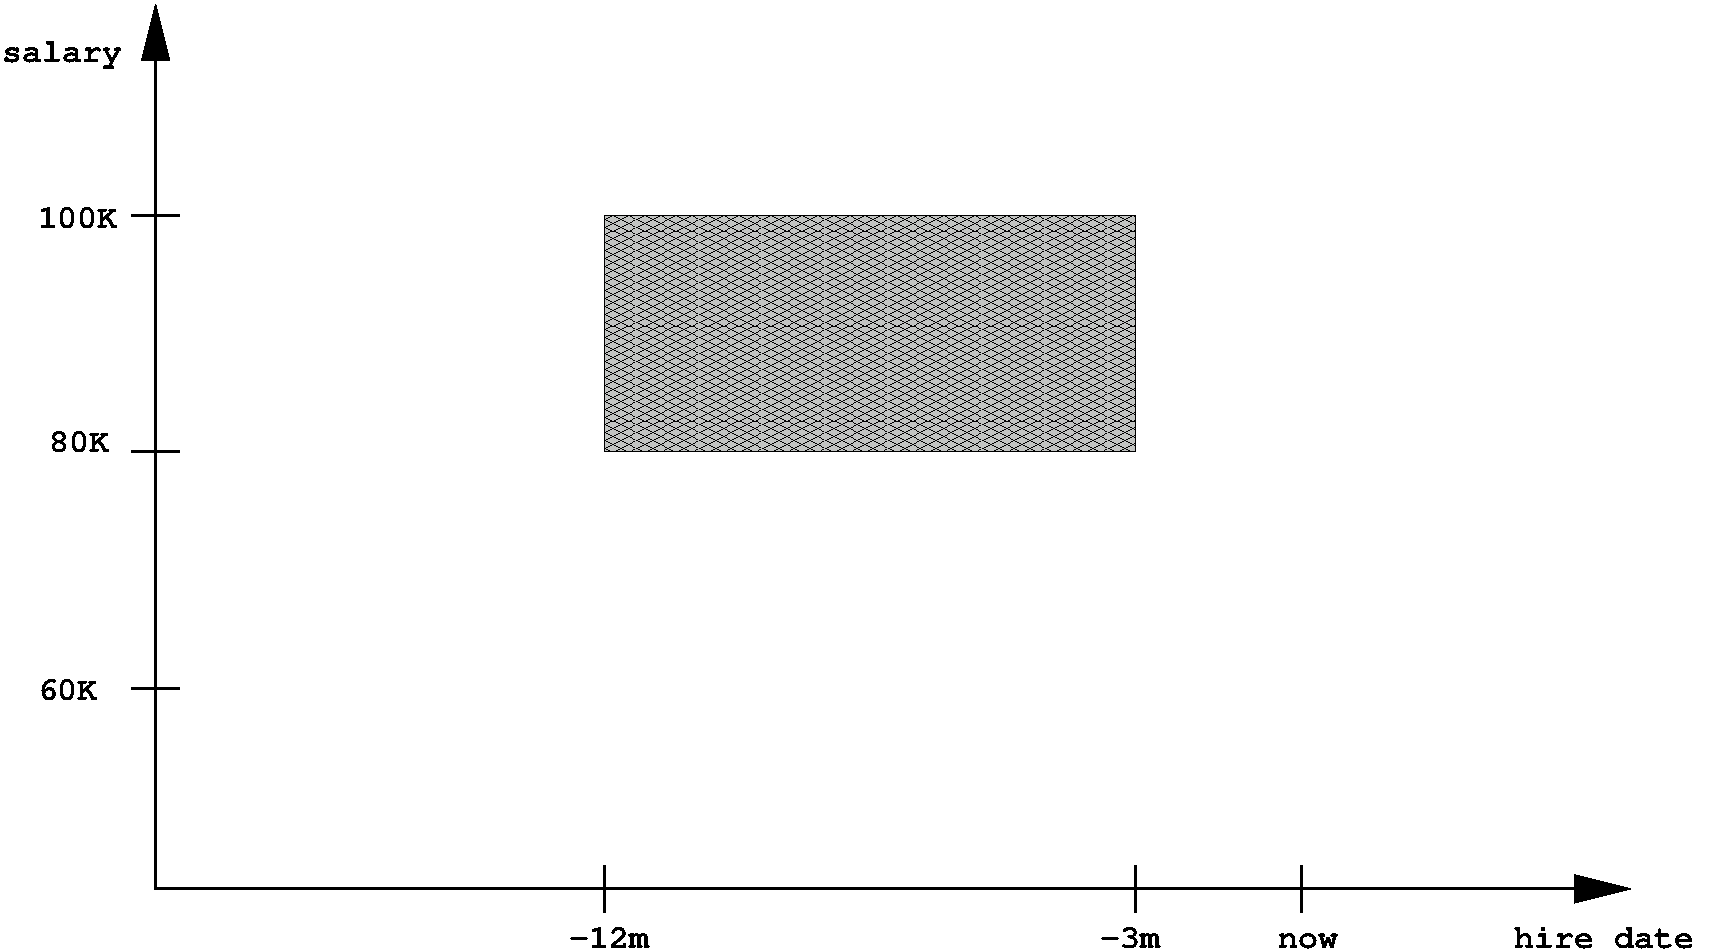
\includegraphics[width=\textwidth]{kd-SQL.pdf}
\end{frame}

\begin{frame}
  \frametitle{Kd-Trees in $\mathbb{R}^1$}
  
  \begin{itemize}
  \item Binary search tree
  \item Find beginning of range
  \item Tree walk to end of range
  \end{itemize}
\end{frame}

\begin{frame}
  \frametitle{Kd-Trees in $\mathbb{R}^2$}
  \begin{itemize}
  \item At root, start with all points.
  \item Partition on $x$ value to make level 1 nodes
  \item Partition those sets on $y$ value to make level 2 nodes
  \item Repeat until done
  \item Result of a query is a forest of subtrees
  \end{itemize}
\end{frame}

\begin{frame}
  \frametitle{Kd-Trees in Pictures}

  \includegraphics<1>[width=.45\textwidth]{kd-tree-0.pdf} 
  \includegraphics<1>[width=.45\textwidth]{kd-tree-graph-0.pdf}
%
  \includegraphics<2>[width=.45\textwidth]{kd-tree-1.pdf}
  \includegraphics<2>[width=.45\textwidth]{kd-tree-graph-1.pdf}
%
  \includegraphics<3>[width=.45\textwidth]{kd-tree-2.pdf}
  \includegraphics<3>[width=.45\textwidth]{kd-tree-graph-2.pdf}
%
  \includegraphics<4>[width=.45\textwidth]{kd-tree-3.pdf}
  \includegraphics<4>[width=.45\textwidth]{kd-tree-graph-3.pdf}
%
  \includegraphics<5>[width=.45\textwidth]{kd-tree-4.pdf}
  \includegraphics<5>[width=.45\textwidth]{kd-tree-graph-4.pdf}
%
  \includegraphics<6>[width=.45\textwidth]{kd-tree-full.pdf}
  \includegraphics<6>[width=.45\textwidth]{kd-tree-graph-5.pdf}
  
\end{frame}

\begin{frame}
  \frametitle{Kd-Trees in Mathematics}
  \begin{itemize}
  \item Split the points into two equal sets with a horizontal separator
  \item If the set has only one point, return a leaf with that point
  \item Else recursively construct a kd-tree on each set, but splitting vertically
  \end{itemize}
  \pause
  \bigskip
  More precisely, split horizontally at odd depth, vertically at even depth.
\end{frame}

\begin{frame}
  \frametitle{Kd-Trees in Equations}
  \begin{itemize}
  \item $O(n)$ storage
  \item $O(n\log n)$ to build
  \item $O(\sqrt{n}+k)$ to query axis-parallel rectangles
  \end{itemize}
\end{frame}

\begin{frame}
  \frametitle{Kd-Trees in Popular Culture}
  \begin{itemize}
  \item Better worst-case behaviour than quadtrees
  \item Bentley, 1975
    \smallgray{(J.~L.~Bentley, Multidimensional binary
      search trees used for associative searching, Communications of
      the ACM, 18:509--517, 1975)}
  \item kNN \smallgray{(for small dimension)}
  \end{itemize}
  \bigskip \gray{M. de Berg et al., \textit{Computational
      Geometry: Algorithms and Applications}, second edition, chapter
    5.  Cf. also chapter end notes.}
\end{frame}

\subsection{Range trees}

\begin{frame}
  \frametitle{Range trees in Words}
  \begin{itemize}
  \item<1-> Range queries again %% JMA
  \item<1-> In $\mathbb{R}^1$, a balanced binary search tree
  \item<2-> In $\mathbb{R}^d$, split on dimension 1 with auxiliary
    range tree on remaining $d-1$ dimensions
  \item<3-> Faster but bigger
  \end{itemize}
\end{frame}

\begin{frame}
  \frametitle{Range trees in Pictures}

  \includegraphics<1>[width=\textwidth]{range-tree-0.pdf} 
  \includegraphics<2>[width=\textwidth]{range-tree-1.pdf} 
  \includegraphics<3>[width=\textwidth]{range-tree-2.pdf} 
  \includegraphics<4>[width=\textwidth]{range-tree-3.pdf} 

\end{frame}

\begin{frame}
  \frametitle{Range trees in Mathematics}

  \begin{itemize}
  \item Build BST on first coordinate: $O(n\log n)$
  \item Recursively build range trees at each interior node on
    remaining $d-1$ coordinates: ??
  \end{itemize}
\end{frame}

\begin{frame}
  \frametitle{Range trees in Equations}
  Compared to kd-trees:
  \begin{itemize}
  \item Faster query times, $O(\log^d n + k)$
  \item Worse storage, $O(n \log^{d-1} n)$
  \item Worse construction,  $O(n\log^{d-1} n)$
  \end{itemize}
\end{frame}

\begin{frame}
  \frametitle{Range trees in Popular Culture}
  \begin{itemize}
  \item Bentley, 1979
    \smallgray{J.~L.~Bentley, Decomposable
      searching problems, Information Processing Letters 8 (5):
      244–251, 1979}
  \item Also: Lueker (1978); Lee, Wong (1980); Willard (1979)
  \end{itemize}

  \bigskip \gray{ 
    M. de Berg et al., \textit{Computational Geometry: Algorithms and
      Applications}, second edition, chapter 5.  Cf. also chapter end
    notes.}
  
  %% Also:
  %
  % Lueker, G. S. (1978). "A data structure for orthogonal range
  % queries". 19th Annual Symposium on Foundations of Computer Science
  % (sfcs 1978). pp. 28–21}
  %
  % Lee, D. T.; Wong, C. K. (1980). "Quintary trees: A file structure
  % for multidimensional database systems". ACM Transactions on
  % Database Systems 5 (3): 339
  %
  % Willard, Dan E. The super-b-tree algorithm (Technical
  % report). Cambridge, MA: Aiken Computer Lab, Harvard
  % University. TR-03-79

\end{frame}

\begin{frame}
  \frametitle{Comparison}

  \begin{tabular}{|l|l|l|l|}
    \hline
    & Space & Time & Query \\
    \hline
    \hline\doublestrut
    quadtree & $O\left(n\log \left(\frac sc\right)\right)$ & $O\left(n\log \left(\frac
      sc\right)\right)$ & $O\left(m\log \left(\frac sc\right)\right)$ \\
    \hline\doublestrut
    kd-tree & $O(n)$ & $O(n\log n)$ & $O(\sqrt n + k)$ \\
    \hline\doublestrut
    range-tree &  $O(n\log^{d-1} n)$ &  $O(n\log^{d-1} n)$ & $O(\log^d n + k)$ \\
    \hline
  \end{tabular}

\end{frame}

\subsection{More}

\begin{frame}
  \frametitle{More\dots}
  \begin{itemize}
  \item Voronoi diagrams
  \item database range searches
  \item kNN \smallgray{\small\it (Use kd-trees for small $d$)}
  \item aNN (locality sensitive hashing)
  \item What if we want to insert or delete points?
  \end{itemize}
\end{frame}

\begin{frame}
  \frametitle{aNN and LSH}

  \begin{itemize}
  \item $N$ points
  \item $h$ hyperplanes, $h \ll N$
  \item planes are oriented
  \item Hamming distance, e.g.
  \end{itemize}
\end{frame}

\begin{frame}
  \frametitle{aNN and LSH}

  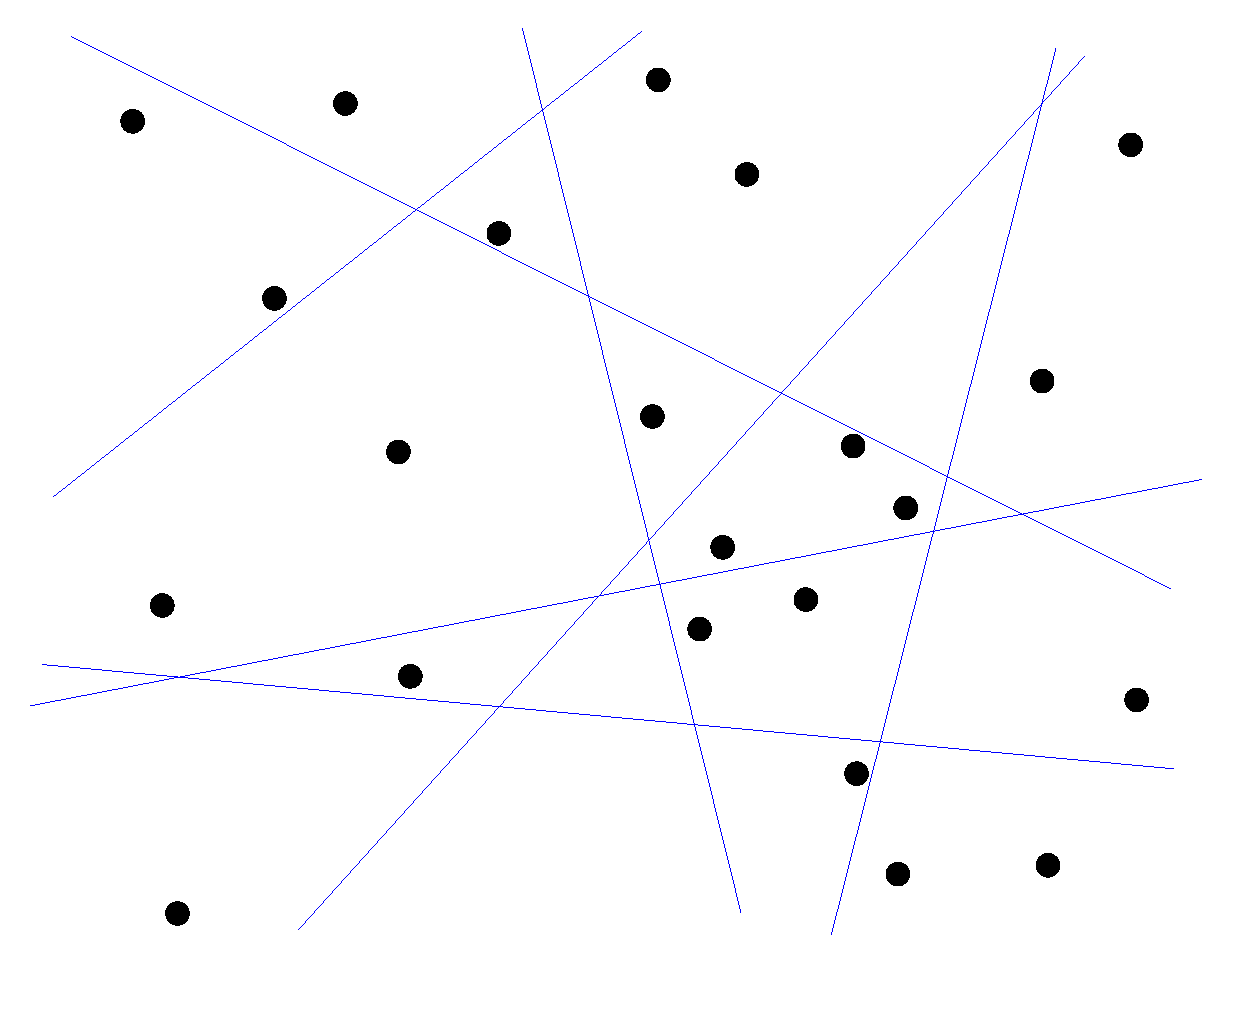
\includegraphics[width=\textwidth]{LSH.pdf}
\end{frame}

\begin{frame}
  \frametitle{Voronoi Diagrams in Words}

  \begin{itemize}
  \item 1-nearest-neighbour
  \item Grass fire function
  \end{itemize}
\end{frame}

\begin{frame}
  \frametitle{Voronoi Diagrams in Pictures}
  \includegraphics<1>[width=.8\textwidth]{voronoi-2a.pdf}
  \includegraphics<2>[width=.8\textwidth]{voronoi-2b.pdf}
\end{frame}

\begin{frame}
  \frametitle{Voronoi Diagrams in Pictures}
  \includegraphics<1>[width=.8\textwidth]{voronoi-circle-a.pdf}
  \includegraphics<2>[width=.8\textwidth]{voronoi-circle-b.pdf}
\end{frame}

\begin{frame}
  \frametitle{Voronoi Diagrams in Pictures}

  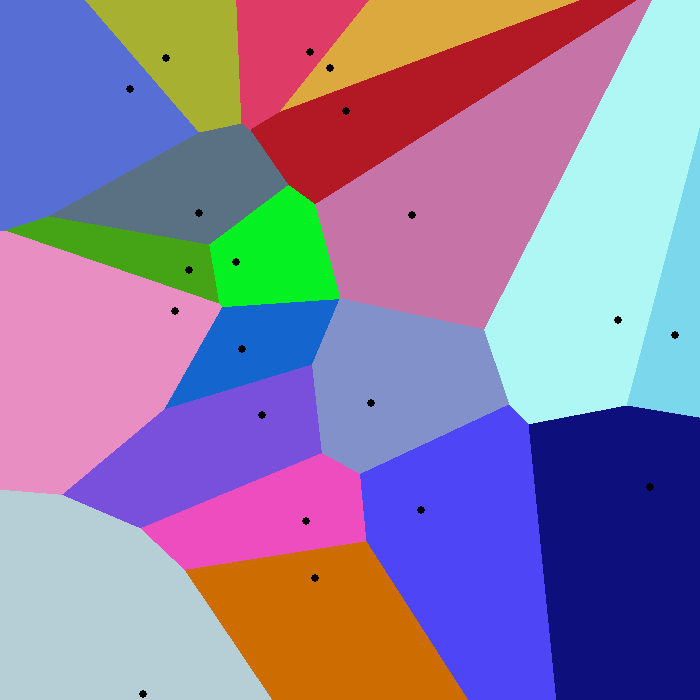
\includegraphics[width=.6\textwidth]{Euclidean_Voronoi_Diagram.png}

  \smallgray{\url{https://en.wikipedia.org/wiki/File:Euclidean_Voronoi_Diagram.png}}
\end{frame}

\begin{frame}
  \frametitle{Voronoi Diagrams in Pictures}

  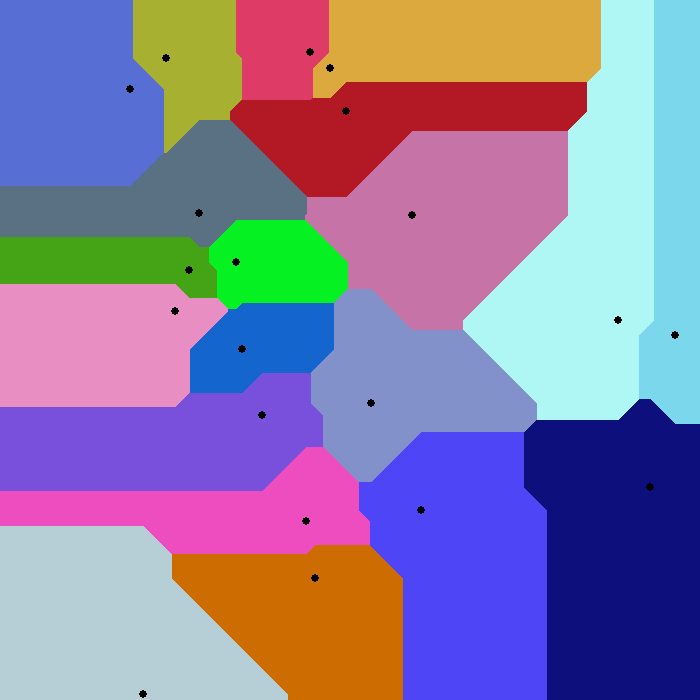
\includegraphics[width=.6\textwidth]{Manhattan_Voronoi_Diagram.png}

  \smallgray{\url{https://en.wikipedia.org/wiki/File:Manhattan_Voronoi_Diagram.png}}
\end{frame}

\begin{frame}
  \frametitle{Voronoi Diagrams in Pictures}

  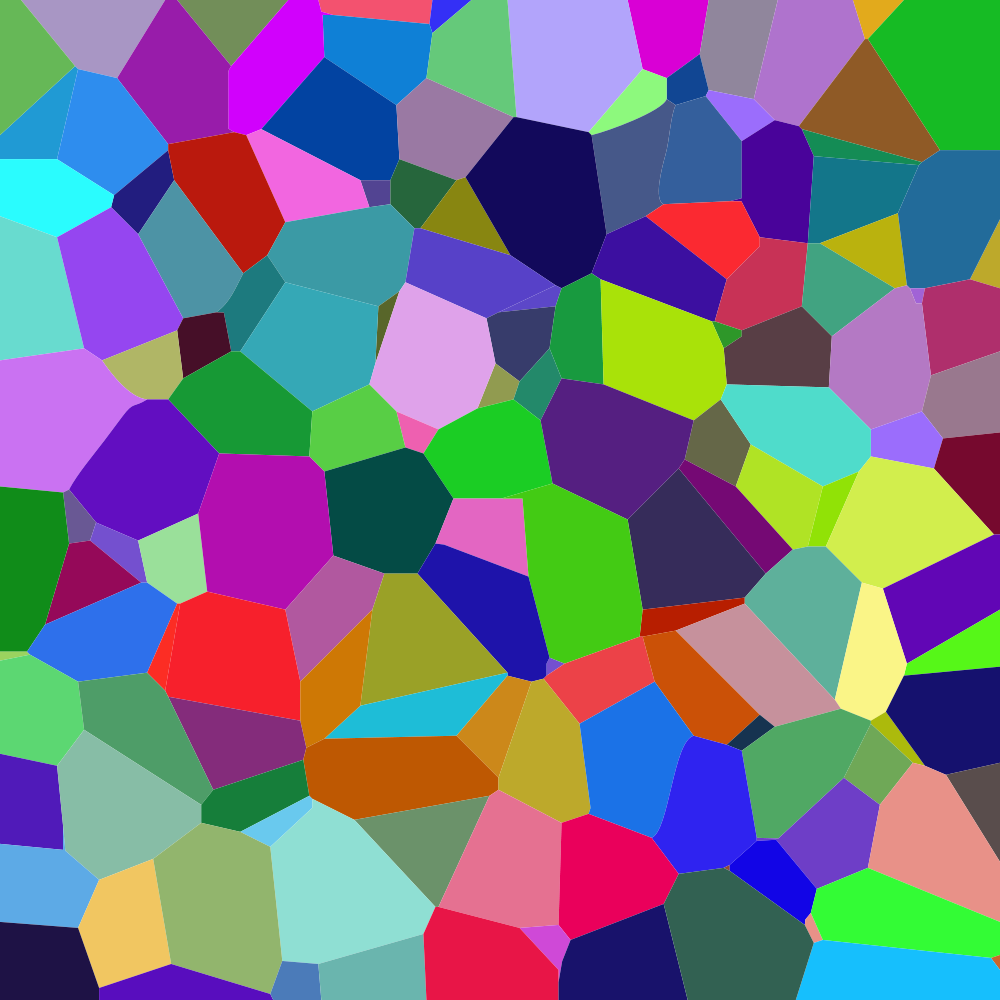
\includegraphics[width=.6\textwidth]{Coloured_Voronoi_3D_slice.png}

  A slice of a 3D voronoi diagram on random points.

  \smallgray{\url{https://en.wikipedia.org/wiki/File:Coloured_Voronoi_3D_slice.svg.png}}
\end{frame}

\begin{frame}
  \frametitle{Voronoi Diagrams in Mathematics}

  \begin{itemize}
  \item Sweep line algorithm
  \item We don't have enough time today\dots
  \end{itemize}
\end{frame}

\begin{frame}
  \frametitle{Voronoi Diagrams in Equations}

  \begin{itemize}
  \item $O(n)$ to store
  \item $O(n\log n)$ to construct
  \end{itemize}
\end{frame}

\begin{frame}
  \frametitle{Voronoi Diagrams in Popular Culture}

  \begin{itemize}
  \item Shamos and Hoey, 1975 \smallgray{(M.I.~Shamos and D.~Hoey,
      Closest-point problems, in Proc. 16th Annual IEEE
      Sympos. Found. Comput. Sci., pp~151--162, 1975)}
  \item Delaunay triangulations \smallgray{(2D)}
  \end{itemize}

  \bigskip \gray{ 
    M. de Berg et al., \textit{Computational Geometry: Algorithms and
      Applications}, second edition, chapter 7.  Cf. also chapter end
    notes.}  

\end{frame}

\section*{Summary}

\begin{frame}
  \frametitle{Summary}  

  \begin{itemize}
  \item Trade-offs
  \item Every problem is different
  \item Dimension matters
  \item This is all quite simplified
  \end{itemize}
\end{frame}

\begin{frame}
  \frametitle{Questions}  
\end{frame}

\end{document}
